\chapter{\IfLanguageName{dutch}{Resultaten}{Resultaten}}
\label{ch:resultaten}
In dit hoofdstuk worden de testen en hun resultaten besproken.
\section{\IfLanguageName{dutch}{Bespreking requirementanalyse}{Analyzing requirementanalyse}}
WACHTEN OP MEER ANTWOORDEN
\section{\IfLanguageName{dutch}{Vergelijking tussen GPS van een gsm en proof of concept}{Difference between the GPS from a phone and the proof of concept}}
Tijdens de eerste test werden er 2 toestellen gebruikt, de proof of concept en een gsm. De gsm is een Xiaomi Mi 9T (kostprijs 332 euro).
Voor de eerste field test is er op voorhand een route uitgestippeld (zie figuur \ref{fig:uitgestippelde_route}). Tijdens het wandelen van deze route stuurde de proof of concept (\ref{ch:proof-of-concept}) en de mobiele applicatie (\ref{ch:mobileapp}) tegelijk hun locaties door om de drie seconden. (Zie figuur \ref{fig:field_test_1})
\begin{figure}
	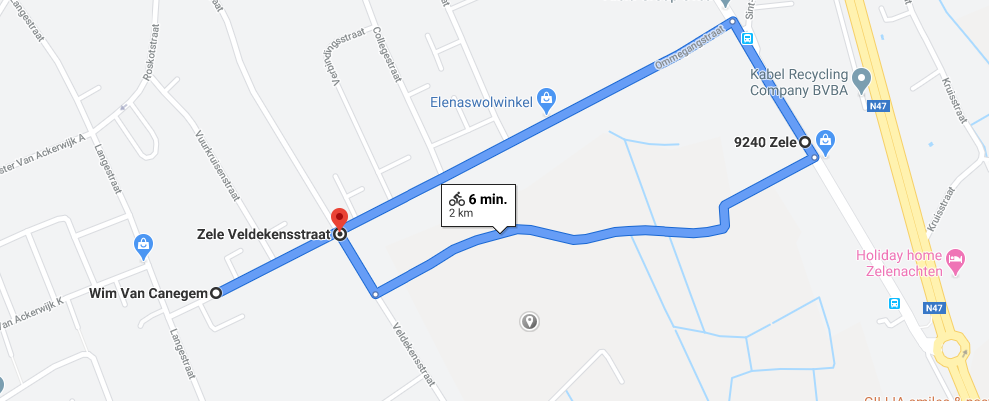
\includegraphics[width=\textwidth,height=\textheight,keepaspectratio]{uitgestippelde_route.png}
	\caption{de uitgestippelde route voor de eerste field test}
	\label{fig:uitgestippelde_route}
\end{figure}
\begin{figure}
	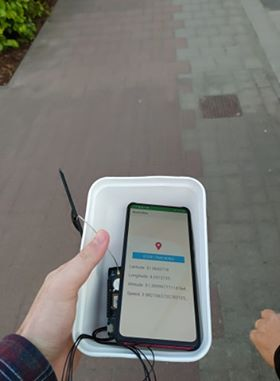
\includegraphics[width=50mm,height=100mm,keepaspectratio]{field_test_1.jpg}
	\caption{Het uitvoeren van de eerste field test}
	\label{fig:field_test_1}
\end{figure}
\begin{figure}
	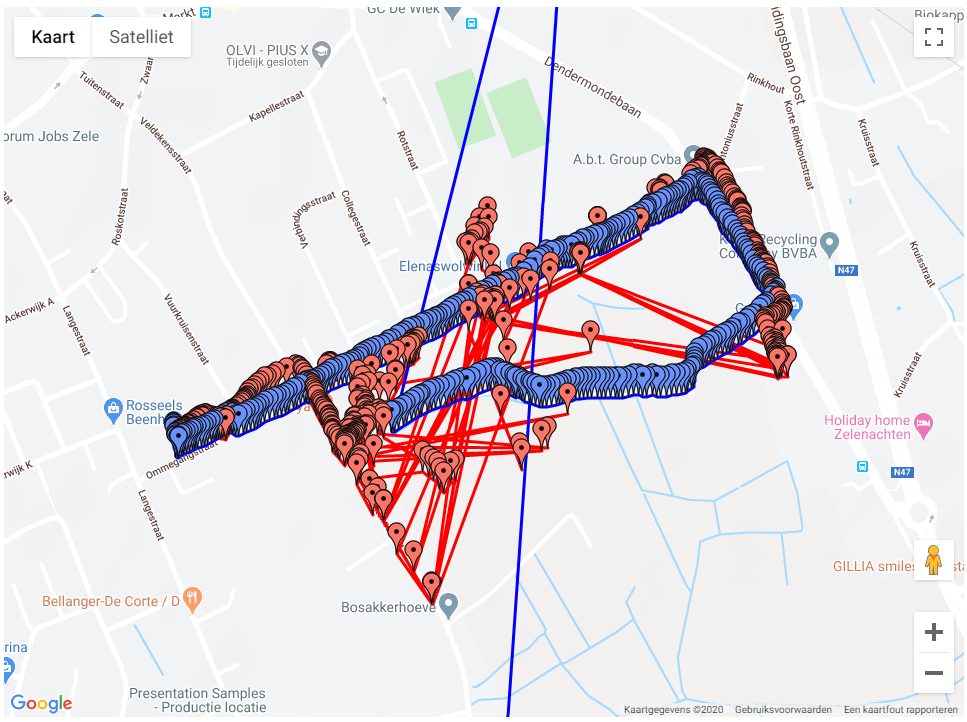
\includegraphics[width=\textwidth,height=\textheight,keepaspectratio]{field_test_1_resultaat.png}
	\caption{Resultaat van de eerste field test}
	\label{fig:field_test_1_resultaat}
\end{figure}
\newline
\newline
Het resultaat is zeer opmerkelijk. In figuur \ref{fig:field_test_1_resultaat} is het duidelijk dat de proof of concept (blauwe markers) beter scoort dan dan de GPS van een gsm (rode markers). De reden hiervoor kan niet volledig verklaart worden, want er kan geen onderzoek gedaan worden naar de GPS-chip in een gsm. Deze data is niet toegankelijk voor ontwikkelaars, alleen voor de fabrikant. De enige data die verkregen kan worden van de GPS-chip is de berekende locatie. 
\newline
Wat opvalt is dat Google Maps wel accuraat lijkt te werken indien de route op de gsm zelf gevolgd wordt. Dit komt omdat Android en iOS extra informatie gebruiken zoals gsm-masten en wifi signalen (SSIDs). Google Maps maakt ook gebruik van verschillende algoritmes om de locatie te corrigeren zodat het lijkt alsof je gsm locatie altijd accuraat is.
\newline
Uit de eerste field test kan er dus geconcludeerd worden dat de proof of concept zijn lokatiebepaling meer accuraat is dan die van een gsm. 